% This file was converted to LaTeX by Writer2LaTeX ver. 1.0.2
% see http://writer2latex.sourceforge.net for more info
\documentclass[twoside,letterpaper]{article}
\usepackage[latin1]{inputenc}
\usepackage[T1]{fontenc}
\usepackage[english]{babel}
\usepackage{amsmath}
\usepackage{amssymb,amsfonts,textcomp}
\usepackage{color}
\usepackage{array}
\newcolumntype{M}[1]{>{\centering\arraybackslash}m{#1}}
\usepackage{supertabular}
\usepackage{hhline}
\usepackage{hyperref}
\usepackage{float}
\hypersetup{pdftex, colorlinks=true, linkcolor=blue, citecolor=blue, filecolor=blue, urlcolor=blue, pdftitle=SOFTWARE REQUIREMENTS SPECIFICATION (SRS), pdfauthor=Shaylyn Adams}
\usepackage[pdftex]{graphicx}
% Outline numbering
\setcounter{secnumdepth}{5}
\renewcommand\thesection{\arabic{section}}
\renewcommand\thesubsection{\arabic{section}.\arabic{subsection}}
\renewcommand\thesubsubsection{\arabic{section}.\arabic{subsection}.\arabic{subsubsection}}
\renewcommand\theparagraph{\arabic{section}.\arabic{subsection}.\arabic{subsubsection}.\arabic{paragraph}}
\renewcommand\thesubparagraph{\arabic{section}.\arabic{subsection}.\arabic{subsubsection}.\arabic{paragraph}.\arabic{subparagraph}}
\makeatletter
\newcommand\arraybslash{\let\\\@arraycr}
\makeatother
% Page layout (geometry)
\setlength\voffset{-1in}
\setlength\hoffset{-1in}
\setlength\topmargin{0.5in}
\setlength\oddsidemargin{1in}
\setlength\evensidemargin{1in}
\setlength\textheight{8.278in}
\setlength\textwidth{6.5in}
\setlength\footskip{0.561in}
\setlength\headheight{0.5in}
\setlength\headsep{0.461in}
% Footnote rule
\setlength{\skip\footins}{0.0469in}
\renewcommand\footnoterule{\vspace*{-0.0071in}\setlength\leftskip{0pt}\setlength\rightskip{0pt plus 1fil}\noindent\textcolor{black}{\rule{0.25\columnwidth}{0.0071in}}\vspace*{0.0398in}}
% Pages styles
\makeatletter
\newcommand\ps@Standard{
  \renewcommand\@oddhead{\selectlanguage{english}\rmfamily\color{black} University of Massachusetts CICS \hfill \hfill Health-e}
  \renewcommand\@evenhead{\@oddhead}
  \renewcommand\@oddfoot{\foreignlanguage{english}{\textcolor{black}{SRS Page }}\foreignlanguage{english}{\textcolor{black}{\thepage{}}}}
  \renewcommand\@evenfoot{\@oddfoot}
  \renewcommand\thepage{\arabic{page}}
}
\newcommand\ps@Convertviii{
  \renewcommand\@oddhead{}
  \renewcommand\@evenhead{\@oddhead}
  \renewcommand\@oddfoot{}
  \renewcommand\@evenfoot{\@oddfoot}
  \renewcommand\thepage{\arabic{page}}
}
\newcommand\ps@Convertvii{
  \renewcommand\@oddhead{}
  \renewcommand\@evenhead{\@oddhead}
  \renewcommand\@oddfoot{}
  \renewcommand\@evenfoot{\@oddfoot}
  \renewcommand\thepage{\arabic{page}}
}
\newcommand\ps@Convertvi{
  \renewcommand\@oddhead{}
  \renewcommand\@evenhead{\@oddhead}
  \renewcommand\@oddfoot{}
  \renewcommand\@evenfoot{\@oddfoot}
  \renewcommand\thepage{\arabic{page}}
}
\newcommand\ps@Convertv{
  \renewcommand\@oddhead{}
  \renewcommand\@evenhead{\@oddhead}
  \renewcommand\@oddfoot{}
  \renewcommand\@evenfoot{\@oddfoot}
  \renewcommand\thepage{\arabic{page}}
}
\newcommand\ps@Convertiv{
  \renewcommand\@oddhead{}
  \renewcommand\@evenhead{\@oddhead}
  \renewcommand\@oddfoot{}
  \renewcommand\@evenfoot{\@oddfoot}
  \renewcommand\thepage{\arabic{page}}
}
\newcommand\ps@Convertii{
  \renewcommand\@oddhead{}
  \renewcommand\@evenhead{\@oddhead}
  \renewcommand\@oddfoot{}
  \renewcommand\@evenfoot{\@oddfoot}
  \renewcommand\thepage{\arabic{page}}
}
\newcommand\ps@FirstPage{
  \renewcommand\@oddhead{}
  \renewcommand\@evenhead{\@oddhead}
  \renewcommand\@oddfoot{}
  \renewcommand\@evenfoot{\@oddfoot}
  \renewcommand\thepage{\arabic{page}}
}
\makeatother
\pagestyle{Standard}
\setlength\tabcolsep{1mm}
\renewcommand\arraystretch{1.3}
% footnotes configuration
\makeatletter
\renewcommand\thefootnote{\arabic{footnote}}
\makeatother
\begin{document}
\clearpage\setcounter{page}{1}\pagestyle{Standard}
\thispagestyle{FirstPage}
\clearpage{\centering\selectlanguage{english}\bfseries\color{black}
SOFTWARE REQUIREMENTS SPECIFICATION (SRS) FOR 
\par}


\bigskip

{\centering\selectlanguage{english}\bfseries\color{black}
320 Green Team Project
\par}


\bigskip


\begin{figure}
\centering

\includegraphics[width=1.5in,height=1.5in]{Uma_seal.png}
\end{figure}

\bigskip


\bigskip

{\centering\selectlanguage{english}\bfseries\color{black}
Version 1.0
\par}

{\centering\selectlanguage{english}\bfseries\color{black}
October 22, 2015
\par}


\bigskip


\bigskip

{\centering\selectlanguage{english}\bfseries\color{black}
Prepared for:
\par}

{\centering\selectlanguage{english}\bfseries\color{black}
Sunderland/Leverett, MA Health Inspector
\par}


\bigskip


\bigskip

{\centering\selectlanguage{english}\bfseries\color{black}
Prepared by:
\par}

{\centering\selectlanguage{english}\bfseries\color{black}
Ather Akhtar, Andrew Chang, Peter Marathas, Andrew Marchetti, \par} 
{\centering\selectlanguage{english}\bfseries\color{black}
 Michael Markman, Eric Maryea, Neven Recchia,
\par}
{\centering\selectlanguage{english}\bfseries\color{black}
Shawn Sowersby, Alex Sullivan, and Josh Tranfaglia.\par}

{\centering\selectlanguage{english}\bfseries\color{black}
University of Massachusetts
\par}

{\centering\selectlanguage{english}\bfseries\color{black}
Amherst, MA \ 01003
\par}


\clearpage{\centering\selectlanguage{english}\bfseries\color{black}
\foreignlanguage{english}{\MakeUppercase{\ }}\foreignlanguage{english}{\MakeUppercase{320 
Green Team Project: Health-e}}
\par}

{\centering\selectlanguage{english}\bfseries\color{black}
TABLE OF CONTENTS
\par}


\bigskip

{\selectlanguage{english}\bfseries\color{black}
Section\ \hfill  Page}

\setcounter{tocdepth}{9}
\renewcommand\contentsname{}
\tableofcontents

\bigskip

\clearpage\clearpage\setcounter{page}{1}\pagestyle{Convertii}
\section[INTRODUCTION]{\selectlanguage{english}\rmfamily\bfseries\color{black}
INTRODUCTION}

\subsection[PURPOSE]{\selectlanguage{english}\rmfamily\bfseries\color{black}
PURPOSE}
{\selectlanguage{english}\rmfamily\color{black}
Convert current, physical method of archiving Board of Health data from restaurant inspections, well water quality tests, and septic tank inspections to a new, digital method.This document provides a high level overview of the entire system then goes into detail on the tablet applications form entry, browsing and search, and delayed upload.
}


\subsection[DOCUMENT CONVENTIONS]{\selectlanguage{english}\rmfamily\bfseries\color{black}
DOCUMENT CONVENTIONS}
{\selectlanguage{english}\rmfamily\color{black}
WRITE HERE}


\subsection[PRODUCT SCOPE]{\selectlanguage{english}\rmfamily\bfseries\color{black}
SCOPE}
{\selectlanguage{english}\rmfamily\color{black}
This project contains multiple sub-projects and systems. 
\\     \\
This new digital method requires a database to hold different types of inspection forms (restaurant, water well, septic tank). The database will be searchable and sortable by keywords or established parameters thus improving accessibility and simplifying analysis. Storing this data digitally will allow the customer to better analyze patterns and create a more permanent location for the data to reside. It will act as an intuitive tool to help the inspector utilize and access data in the future. To increase usability of this database, a user interface must be created to provide access and retrieval of information. This application will focus on usability of the database and a later described portion will focus on portability, thus one can think of this application as residing in an office environment. The application should include a convenient and easy method to search, sort, and analyze data from the restaurant inspections, well water quality reports, and septic tank inspections. Septic tank and well water quality inspection data should also be viewable on a geographical map with the ability to show change over time. This will illuminate differences and trends in the data that may help explain and predict the cause of said trends. The cataloguing of restaurant health inspection data could be facilitated by a form on a portable application (i.e. mobile, tablet). This portable application should be designed to locally store the inputted data and convert it to a form readable by the database so it can add the report to the rest of the database when connected. Overall, creating and structuring this database for the customer and providing easy-to-use tools for accessing it, will assist him in his inspections and simplify the retrieval of key information the customer might be interested in at a later date.
\subsubsection{Sub Projects}
\begin{itemize}
\item{Central Database}
\item{Form Application for Tablet}
\item{Application}
\end{itemize}
\textit{Central Database:}
\newline 

A central database with consistent access to data will create the integrity of the entire system. The three distinct data entities identified were: Well water inspections, septic tank inspections, and restaurant inspections, which will all need to contain location to differentiate towns. The attributes of the models will correspond to the required fields that the customer must fill in on their forms during inspections. The data for the restaurant inspections shall contain all fields that can be found on the restaurant inspection form. The data for water inspections must contain all of the relevant fields, such as water quality, measurements, address of water well, flow rate, name of the company that drilled the well, and the permit and lot number. Similarly, the data for the septic inspection will hold information such as the address, lot number, size, capacity, condition of the tank, date of last inspection, and quality of gallons pumped in and out.  The type of data stored must be able to be changed in the event of new legislation.
\newline

The two features existing in the database include a basic database that provides basic queries to GET, POST, PUT, and DELETE records safely and securely. The other feature is to create and design a federated database.
\\  \\
\textit{Form Application for a Tablet:}
\newline

This application will be focused on usability in attempt to make it as simple as possible to enter form data. The application will be able to store data locally on the device followed by having the ability to upload to the office-based application noted (i.e. desktop application or web -application). This app will replicate the forms that the customer requires for every inspection For security reasons, the app will have a login screen for user authentication. This application will be able to either send the document to a printer or email it on the spot as well as being able to receive an e-signature. The application should allow the user to view contextual information based on data that is associated with the users current task. For example, when the user is going to inspect a restaurant, they should be shown previous inspection results. 
\newline

The form application will have the following main areas that correspond with the functionality above. User authentication as stated. Data entry as stated where the user interface allows the inspector to flow through the inspection process dynamically. Data entry (GIS) is required in order to locate well, septic, and restaurant location. Form printing is another important point as a physical copy of a restaurant inspection will most likely be required to provide to the restaurant owner. Browsing and search is also a feature of the application which includes pulling up relevant data of a current restaurant. The final important feature is the ability for delayed upload. This will allow the tablet to flow data into the central database that communicates with the main application on the web.
\\ \\
\textit{Application (Usable, Connected to Database):}
\newline

An application will be created for viewing all past records stored in the database. The application should include three different sections for restaurant, water and septic.  The application will need to communicate with the central databases containing all information of past record. The site will provide an interface for querying data, including searching by location or violation. The application will contain user authentication that, once validated for an administrator, will allow for the submission of new records. Without login credentials, the information is read-only. The site will use the accepted regulation form as a base to record data from a new restaurant, water, or septic inspection and then send this new data to the relevant database. Additional functionality including mapping is mentioned next.
\newline 

Features described have included user authentication, data entry for eligible users, reporting and search as well as mapping. The reporting and search will include the ability to retrieve a general summary of 1 of 3 sections (restuarants, wells, septic tanks) that will be able to be downloaded and printed for use in a physical report. The application will also include data mapping. This map will contain points of location of wells, septic tanks, and restaurants which can then be queried and visualized. }

\subsection[INTENDED AUDIENCE]{\selectlanguage{english}\rmfamily\bfseries\color{black}
INTENDED AUDIENCE}
{\selectlanguage{english}\rmfamily\color{black}
    The intended audience is for health inspectors who want to use a digital alternative to record and store information as an alternative to physical methods. The primary audience will be the health inspector of the town of Leverett and Sunderland Massachusetts.}

\subsection[DEFINITIONS, ACRONYMS, AND
ABBREVIATIONS]{\selectlanguage{english}\rmfamily\bfseries\color{black}
DEFINITIONS, ACRONYMS, AND ABBREVIATIONS}
{\selectlanguage{english}\rmfamily\color{black}
The products name is Health.e standing for Health electronics as it is designed to digitize information on health inspections, well water and septic tanks.}
\newline
\begin{flushleft}
\tablehead{}
\begin{supertabular}{|m{1.3587599in}|m{5.00806in}|}
\hline
\centering \selectlanguage{english}\bfseries\color{black} Term or
Acronym &
\centering\arraybslash \selectlanguage{english}\bfseries\color{black}
Definition\\\hline
\selectlanguage{english}\color{black} Alpha test &
\selectlanguage{english}\color{black} Limited release(s) to selected,
outside testers\\\hline
\selectlanguage{english}\color{black} Beta test &
\selectlanguage{english}\color{black} Limited release(s) to cooperating
customers wanting early access to developing systems\\\hline
\selectlanguage{english}\color{black} Final test &
\selectlanguage{english}\color{black} aka, Acceptance test, release of
full functionality to customer for approval\\\hline
\selectlanguage{english}\color{black} DFD &
\selectlanguage{english}\color{black} Data Flow Diagram\\\hline
\selectlanguage{english}\color{black} SDD &
\selectlanguage{english}\color{black} Software Design Document, aka SDS,
Software Design Specification\\\hline
\selectlanguage{english}\color{black} SRS &
\selectlanguage{english}\color{black} Software Requirements
Specification\\\hline
\selectlanguage{english}\color{black} SSRS &
\selectlanguage{english}\color{black} System and Software Requirements
Specification\\\hline
~
 &
~
\\\hline
~
 &
~
\\\hline
~
 &
~
\\\hline
~
 &
~
\\\hline
\end{supertabular}
\end{flushleft}

% \subsection[REFERENCESS]{\selectlanguage{english}\rmfamily\bfseries\color{black}
% REFERENCES}
% {\selectlanguage{english}\itshape\color{black}
% WRITE HERE}


\clearpage\section[OVERALL
DESCRIPTION]{\selectlanguage{english}\rmfamily\bfseries\color{black}
OVERALL DESCRIPTION}

\subsection[PRODUCT
PERSPECTIVE]{\selectlanguage{english}\rmfamily\bfseries\color{black}
PRODUCT PERSPECTIVE}
This product, in all of its glory, will be replacing the primary user's current pen and paper system for documenting inspection forms. Rather than filling out paper forms on site and handing the inspectee a carbon copy of the form, the tablet app will allow the inspector to fill out a digitalized version of the same form, and print said form from a wireless printer on site for the inspectee to obtain. Also, rather than storing paper files in a filing cabinet that may never be looked at again, the health inspector may, with our product, review previous forms with ease by searching for them with our comprehensive browsing and search functionality. This way, files may be found in a matter of seconds. Another aspect of this product will be the delayed upload in which forms that have been filled out on the tablet and stored locally will be synced with the central database so that they may be integrated with the main application. This eliminates the need for the health inspector to ''file'' each form after completing it.
\newline
The form entry, browsing and search, and delayed upload functionalities are all subprojects for the entire tablet app, which is, in and of itself, a subproject of the main project. Our contribution to the main project is depicted below:

\begin{figure}[H]
\centering
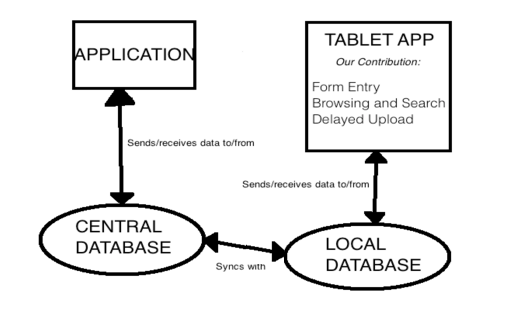
\includegraphics[width=4in,height=3in]{Diagram1.png}
\end{figure}


\subsection[PRODUCT
FUNCTIONS]{\selectlanguage{english}\rmfamily\bfseries\color{black}
PRODUCT FUNCTIONS}
\subsubsection{Data Entry (Form)}
\begin{enumerate}
\item{The user chooses one of the following inspection forms to fill in: restaurant, septic tank, or water well.}
\item{The tablet then displays the chosen form to the user with blank, fillable forms.}
\end{enumerate}
\subsubsection{Browsing \& Search}
\begin{enumerate}
\item{The user types in a location of the desired restaurant, septic tank, or water well.}
\item{The tablet displays forms from its database relevant to the search requirements.}
\end{enumerate}
\subsubsection{Delayed Upload}
\begin{enumerate}
\item{The tablet synchronizes with the external database and uploads either specific or all form entries from the tablet to the external database once a connection has been established.}
\end{enumerate}

\subsection[USER
CHARACTERISTICS]{\selectlanguage{english}\rmfamily\bfseries\color{black}
USER CHARACTERISTICS}
{\selectlanguage{english}\rmfamily\color{black}
The form entry, browsing and search, and delayed upload parts of the tablet will primarily be used by health inspectors. They will have full access to all functional aspects listed in section 2.2. Unregistered guests will have limited, read-only access to the main application of the project while only the registered health inspectors may access the tablet application.}

\subsection[OPERATING ENVIRONMENT]{\selectlanguage{english}\rmfamily\bfseries\color{black}
OPERATING ENVIROMENT}
{\selectlanguage{english}\rmfamily\color{black}
The form entry, browsing and search, and delayed upload aspects of this project will all exist on the same platform: a tablet. The tablet should have a small amount of memory allocated to the app so that data forms may be stored locally until uploaded to the central database.}



\subsection[CONSTRAINTS]{\selectlanguage{english}\rmfamily\bfseries\color{black}
CONSTRAINTS}
\subsubsection{Data Entry (Form)}
{\selectlanguage{english}\color{black}
The form entry itself is primarily based on inspection forms created by the state and used by the town. The entry fields on each form entry in the tablet has to match the required sections on the current inspection forms. Also, there will be a finite amount of form entries the user could generate with the tablet since the tablet will have a limited amount of memory space. With recent tablet device improvements, the chances of filling up the memory on the tablet is low. With a good design of the entire project, modern day memory capacities will suffice to hold the data required.}

\subsubsection{Browsing \& Search}
{\selectlanguage{english}\color{black}
Browsing and searching features are constrained by the design of the database itself. With a good design and structure, these features will be user intuitive and minimal effort will be needed by the user to use these features. Browsing and searching the form entries is constrained by the number of form entries in the database on the tablet.}

\subsubsection{Delayed Upload}
{\selectlanguage{english}\color{black}
The delayed upload is constrained by the health inspector's access to WiFi or some form of manual docking technology. Either method may be used in order for the local memory on the tablet to sync with the central database, but one must exist.}

\subsection[USER DOCUMENTATION]{\selectlanguage{english}\rmfamily\bfseries\color{black}
USER DOCUMENTATION}
{\selectlanguage{english}\rmfamily\color{black}
There will be a GitHub Wiki that will help guide the user through all of the basic functionality of the tablet app, and in general, the application as a whole. The Wiki will be user friendly, easily comprehensible, and will touch on all of the important features of the app that the primary user should be familiar with.}

\subsection[ASSUMPTIONS \& DEPENDENCIES]{\selectlanguage{english}\rmfamily\bfseries\color{black}
ASSUMPTIONS \& DEPENDENCIES}
\subsubsection{Data Entry (Form)}
Our implementation of the form entry on the tablet app depends on how the central database is constructed. Each field that the database contains for each type of form must be represented in the UI of the tablet app so that the health inspector may enter all of the fields correctly. The assumption here being that any changes made to the physical forms will be updated accordingly in the database, and thus updated in the digital forms as well. 
\subsubsection{Browsing \& Search}
Our implementation of browsing and search on the tablet app relies partly on the implementation of the database since fields that will ultimately be searched for within the tablet app must be connected to the database in some form. However, the only main assumption for this aspect of the project is that the files being searched for still exist on the tablet. There is a possibility that files that have been removed from the tablet may be searched for, but such a case will be handled by a file not found message. 
\subsubsection{Delayed Upload}
We are assuming that the health inspector will have WiFi access in order for the tablet app to upload data from its local database to the central database via a syncing process. In the case that this assumption is incorrect and the user does not have WiFi access, a manual docking process will have to occur between the tablet and the health inspector's computer on which the main application exists. This assumes that the health inspector has the proper cable to connect the tablet to said computer, but this is a reasonable assumption since such a cable typically is included with the purchase of a tablet since its serves the dual purpose of a charger. The delayed upload also depends on the construction of the database and its fields as well as the application itself since it must sync with said application.

\clearpage\section[EXTERNAL INTERFACE
REQUIREMENTS]{\selectlanguage{english}\rmfamily\bfseries\color{black}
EXTERNAL INTERFACE
REQUIREMENTS}

\subsection[USER INTERFACES]{\selectlanguage{english}\rmfamily\bfseries\color{black}
USER INTERFACES}
{\selectlanguage{english}\rmfamily\color{black}
The user interface for the system will be an app based application on a tablet. The user will enter information to pass the user authentication. The user will then be able to select which forms to access. The user will be able to enter form data in the app on the replicated forms for the inspection. The user will also be able to send the document to a printer or email it. The user will also be able to accept e-signatures directly inside the app. The app will also have the ability for the user to browse and search for information on the app. The user will be able to select for a delayed upload as well.}

\subsection[HARDWARE INTERFACES]{\selectlanguage{english}\rmfamily\bfseries\color{black}
HARDWARE INTERFACES}
{\selectlanguage{english}\rmfamily\color{black}
  The hardware interfaces of the system will be run on an android device. An internet connection to allow the software interfaces to connect to the internet to sync with files in the database. }

\subsection[SOFTWARE INTERFACES]{\selectlanguage{english}\rmfamily\bfseries\color{black}
SOFTWARE INTERFACES}
{\selectlanguage{english}\rmfamily\color{black}
\subsubsection{Operating System} 
The software is being designed to run on Android OS.
\subsubsection{Web Server}
The software will be able to sync with a database
\subsubsection{Database}
The software will use a federated database to store all the data.}

\subsection[COMMUNICATION INTERFACES]{\selectlanguage{english}\rmfamily\bfseries\color{black}
COMMUNICATION INTERFACES}
{\selectlanguage{english}\rmfamily\color{black}

\subsubsection{Form Interface}
The application will provide electronic forms that the user needs.

\subsubsection{Web Communication}
The application will be able to wirelessly sync with the database.

\subsubsection{USB Communication}
The application will be able to sync through a usb cable with the database.}

\clearpage\section[NONFUNCTIONAL REQUIREMENTS]{\selectlanguage{english}\rmfamily\bfseries\color{black}
NONFUNCTIONAL REQUIREMENTS}
{\selectlanguage{english}\rmfamily\color{black}

\subsection{PERFORMANCE REQUIREMENTS}
For the tablet application, the user expects to experience appropriate speed performance. The focus here is browsing and searching. Getting information from the database should never operate at a speed that will keep the user waiting. 

\subsection{SAFETY REQUIREMENTS}
When it comes to the tablet applications ability to do delayed uploading, safety becomes a factor. Its essential that the data entered on site with the tablet is properly indexed and saved. The tablet must make it back to the users desktop without any loss of this data. 

\subsection{SECURITY REQUIREMENTS}
Its vital that data entry is allowed only to authorized users. User authentication should take care of this, and only let administrators actually enter information into the database. However, we shouldn't have worry about browsing and search, as anyone can use the feature because the information is public.

\subsection{SOFTWRE QUALITY ATTRIBUTES}
The biggest goal here is that the tablet application is extremely user friendly. From what we know, the client who is going to be using the application is not tech-savvy. Between the user interface and functionality, the highlight must be that the user can easily learn how to use the application effectively.

\subsection{BUSINESS ROLES}
Any user with access to the tablet application can do browsing and searching for information on the wells, septic systems and restaurants. All of this information is public. However, only a registered administrator is allowed to access the form entry and delayed upload features. They are the sole owners of the ability to add new information.}

\clearpage\section[FUNCTIONAL REQUIREMENTS]{\selectlanguage{english}\rmfamily\bfseries\color{black}
FUNCTIONAL REQUIREMENTS}
\subsection[DATA ENTRY (FORMS)]{\selectlanguage{english}\rmfamily\bfseries\color{black}
DATA ENTRY (FORMS)}

\subsubsection{\textit{Use Case 1}}

\textit{Title: }{\selectlanguage{english}\bfseries\color{black} Fill out septic tank inspection form}

{\selectlanguage{english}\color{black} \textit{Primary Actor:} User}

{\selectlanguage{english}\color{black} \textit{Secondary Actor:} System}

{\selectlanguage{english}\color{black} \textit{Trigger:} User selects septic inspection form.}

{\selectlanguage{english}\color{black} \textit{Precondition:} User  successfully logged in and accessed the form entry user interface for the septic tank.}

{\selectlanguage{english}\color{black} \textit{Postcondition:}  Data is stored to be submitted to a central database}
\newline

{\selectlanguage{english}\color{black} \textit{Main Scenario:}}
\begin{enumerate}
\item System presents modifiable septic tank information form.

\item User fills out each required field of the form.

\item User submits the form on tablet.

\item System determines that each required and non-required field entered is valid.

\item System creates an accessible local copy.

\item System displays a response when successfully entering form.

\item User safely closes out of process (data is preserved).
\end{enumerate}

{\selectlanguage{english}\color{black} \textit{Exception Scenario:}}
\begin{enumerate}
\item User forgets to enter information in 'required field'.
\begin{enumerate}
\item System notifies user of empty fields and does not submit.
\end{enumerate}

\item User enters an invalid form entry.
\begin{enumerate}
\item System displays invalid form entry and does not submit.
\end{enumerate}

\item System shuts down during data submission.
\begin{enumerate}
\item System can show user whether or not data was submitted successfully. 
\end{enumerate}
\end{enumerate}

\subsubsection{\textit{Use Case 2}} 

\textit{Title: }{\selectlanguage{english}\bfseries\color{black} Fill out well water inspection form}

{\selectlanguage{english}\color{black} \textit{Primary Actor:} User}

{\selectlanguage{english}\color{black} \textit{Secondary Actor:} System}

{\selectlanguage{english}\color{black} \textit{Trigger:} User selects well water inspection form.}

{\selectlanguage{english}\color{black} \textit{Precondition:} Successfully logged in and accessed the form entry user interface for water well inspection.}

{\selectlanguage{english}\color{black} \textit{Postcondition:}  Data is stored to be submitted to a central database}
\newline

{\selectlanguage{english}\color{black} \textit{Main Scenario:}}
\begin{enumerate}
\item System presents modifiable well water information form.

\item User fills out each \textit{required} field of the form.

\item User submits the form on tablet.

\item System determines that each required and non-required field entered is valid.

\item System allocates memory and creates an accessible local copy.

\item System displays a response when successfully entering form.

\item User safely closes out of process (data is preserved).
\end{enumerate}

{\selectlanguage{english}\color{black} \textit{Exception Scenarios:}}
\begin{enumerate}
\item User forgets to enter information in 'required field'.
\begin{enumerate}
\item System notifies user of empty fields and does not submit.
\item User presented with partially filled out form.
\end{enumerate}

\item User enters an invalid form entry.
\begin{enumerate}
\item System displays invalid form entry and does not submit.
\item User presented with partially filled out form.
\end{enumerate}

\item System shuts down during data submission.
\begin{enumerate}
\item System shows user whether or not data was submitted successfully.
\end{enumerate}
\end{enumerate}

\subsubsection{\textit{Use Case 3}}

\textit{Title: }{\selectlanguage{english}\bfseries\color{black} Fill out restaurant inspection form}

{\selectlanguage{english}\color{black} \textit{Primary Actor:} User}

{\selectlanguage{english}\color{black} \textit{Secondary Actor:} System}

{\selectlanguage{english}\color{black} \textit{Trigger:} User selects restaurant inspection form to fill out.}

{\selectlanguage{english}\color{black} \textit{Precondition:} User has passed login authentication, and has chosen to submit data for a restaurant inspection.}

{\selectlanguage{english}\color{black} \textit{Postcondition:}  Data is stored to be submitted to a central database}
\newline

{\selectlanguage{english}\color{black} \textit{Main Scenario:}}
\begin{enumerate}
\item The page for restaurant inspection form is shown.
\item User records location and name of restaurant
\item User fills out fields in form to record data form inspection
\item User clicks save button.
\item Data is stored locally
\end{enumerate}

{\selectlanguage{english}\color{black} \textit{Exception Scenario:}}
\begin{enumerate}
\item User forgets to enter information in 'required field'.
\begin{enumerate}
\item System notifies user of empty fields and does not submit.
\item User presented with partially filled out form.
\end{enumerate}

\item User enters an invalid form entry.
\begin{enumerate}
\item System displays invalid form entry and does not submit.
\item User presented with partially filled out form.
\end{enumerate}

\item System shuts down during data submission.
\begin{enumerate}
\item System shows user whether or not data was submitted successfully. 
\end{enumerate}
\end{enumerate}

\subsection[BROWSING \& SEARCH]{\selectlanguage{english}\rmfamily\bfseries\color{black}
BROWSING \& SEARCH}

\subsubsection{\textit{Use Case 1}}

\textit{Title: }{\selectlanguage{english}\bfseries\color{black} Search for prior inspection report}

{\selectlanguage{english}\color{black} \textit{Primary Actor:} User}

{\selectlanguage{english}\color{black} \textit{Secondary Actor:} System}

{\selectlanguage{english}\color{black} \textit{Trigger:} User wants to search for a list of inspection reports matching an entered keyword.}

{\selectlanguage{english}\color{black} \textit{Preconditions:} User has logged in and is on the inital lookup report screen which contains a list of all inspection reports.}

{\selectlanguage{english}\color{black} \textit{Postcondition:} System displays list of prior reports matching search term.}
\newline

{\selectlanguage{english}\color{black} \textit{Main Scenario:}}
\begin{enumerate}
\item User enters a keyword to search
\item System queries external database with location and retrieves records that contain the keyword
\item System displays a list of retrieved records and their dates, sorted by date
\end{enumerate}

{\selectlanguage{english}\color{black} \textit{Exception Scenarios:}}
\begin{enumerate}
\item System cannot connect to database
\begin{enumerate}
\item Screen displays connection error message and asks user to try again later
\item User selects 'Ok' button and system returns to the lookup report screen
\end{enumerate}

\item None of the records match the search keyword
\begin{enumerate}
\item Display message, ''No reports match the specified keyword''
\item User clicks 'Ok' and returns to the initial lookup report screen
\end{enumerate}
\end{enumerate}

\subsubsection{\textit{Use Case 2}}

\textit{Title: }{\selectlanguage{english}\bfseries\color{black}Narrow down list of inspection reports}

{\selectlanguage{english}\color{black} \textit{Primary Actor:} User}

{\selectlanguage{english}\color{black} \textit{Secondary Actor:} System}

{\selectlanguage{english}\color{black} \textit{Trigger:} User wants to select criteria to narrow down a list of all inspection reports.}

{\selectlanguage{english}\color{black} \textit{Preconditions:} User has logged in and is on the initial lookup report screen which contains a list of all inspection reports.}

{\selectlanguage{english}\color{black} \textit{Postcondition:} System displays list of prior reports matching the selected criteria.}
\newline
{\selectlanguage{english}\color{black} \textit{Main Scenario:}}\
\begin{enumerate}
\item User selects criteria to narrow down all the inspection reports
\item System queries external database with location and retrieves records that match the criteria
\item System displays a list of retrieved records and their dates, sorted by date
\end{enumerate}
{\selectlanguage{english}\color{black} \textit{Exception Scenarios:}}
\begin{enumerate}
\item System cannot connect to database
\begin{enumerate}
\item Screen displays connection error message and asks user to try again later
\item User selects 'Ok' button and system returns to the lookup report screen
\end{enumerate}

\item None of the records match the search keyword
\begin{enumerate}
\item Display message, ''No reports matching that criteria''
\item User clicks 'Ok' and returns to the initial lookup report screen
\end{enumerate}
\end{enumerate}

\subsubsection{\textit{Use Case 3}}

\textit{Title: }{\selectlanguage{english}\bfseries\color{black}View an inspection report}

{\selectlanguage{english}\color{black} \textit{Primary Actor:} User}

{\selectlanguage{english}\color{black} \textit{Secondary Actor:} System}

{\selectlanguage{english}\color{black} \textit{Trigger:} User wants to view a specific inspection report.}

{\selectlanguage{english}\color{black} \textit{Preconditions:} User has logged in and is on the lookup report screen which contains a list inspection reports.}

{\selectlanguage{english}\color{black} \textit{Postcondition:} System displays the selected inspection report.}
\newline
{\selectlanguage{english}\color{black} \textit{Main Scenario:}}\
\begin{enumerate}
\item User selects an inspection report
\item System displays all data contained in the selected inspection report
\end{enumerate}
{\selectlanguage{english}\color{black} \textit{Exception Scenario:}}

\begin{description}
\item System cannot connect to database
\begin{enumerate}
\item Screen displays connection error message and asks user to try again later
\item User selects 'Ok' button and system returns to the lookup report screen
\end{enumerate}
\end{description}

\subsection[DELAYED UPLOAD]
{\selectlanguage{english}\rmfamily\bfseries\color{black}
DELAYED UPLOAD}
\subsubsection{\textit{Use Case 1}}

\textit{Title: }{\selectlanguage{english}\bfseries\color{black}User attempts to upload a specific piece of form data.}

{\selectlanguage{english}\color{black} \textit{Primary Actor:} System}

{\selectlanguage{english}\color{black} \textit{Secondary Actor:} User}

{\selectlanguage{english}\color{black} \textit{Trigger:} User selects septic inspection form to fill out.}

{\selectlanguage{english}\color{black} \textit{Precondition:}User has completed and saved some type of form data, and is associated with some online database. User is on the start page and has signed in successfully. Alternatively, User opts to send form data immediately after saving to device and begins at step 2.}

{\selectlanguage{english}\color{black} \textit{Postcondition:}Form data has not already been submitted to the database and is added successfully. If conditions are not correct for proper form data upload, data is not uploaded.}
\newline

{\selectlanguage{english}\color{black} \textit{Main Scenario:}}
\begin{enumerate}
\item User navigates the form data on the application to find the data they desire to upload.
\item User indicates that they want to upload the form data.
\item System verifies that the form data is acceptable for submission to online database.
\item System verifies that internet connection is available.
\item System verifies that connection to associated database is available.
\item System verifies that given form data has not already been submitted to the database.
\item System asks the user for confirmation to send the form data.
\item User gives confirmation of intent to send the form data
\item System adds the new form data to the database using the internet connection available.
\item System notifies the user of successful upload of the data.
\end{enumerate}

{\selectlanguage{english}\color{black} \textit{Exception Scenario:}}

\begin{enumerate}
\item Form data is not acceptable for upload.
\begin{enumerate}
\item System notifies the user that the form data is not acceptable for upload. System 
specifies which fields in the form data are unacceptable and asks that they be fixed before submission.
\item User is returned to the form's viewing page.
\end{enumerate}

\item No internet connection is available.
\begin{enumerate}
\item System notifies the user that internet connection is not available and to try again once they are within access range.
\item User is returned to the form's viewing page.
\end{enumerate}

\item Only internet connections that are available are not Wi-Fi connections.
\begin{enumerate}
\item System asks the user to verify that they would like to send the connection on the mobile network.
\item If user accepts, use case proceeds as normal at step 4.
\item If user refuses, system notifies the user to try uploading again once they are within access range.
\item User is returned to the form's viewing page.
\end{enumerate}

\item System is unable to connect with the database.
\begin{enumerate}
\item System notifies the user that it is impossible to connect to the database and to verify that the database is online.
\item User is returned to the form's viewing page.
\end{enumerate}

\item Form data has already been submitted to the database.
\begin{enumerate}
\item System notifies the user that the form has already been uploaded before.
\item User is returned to the form's viewing page.
\end{enumerate}

\item User declines the confirmation to send the data.
\begin{enumerate}
\item Form data is not sent. User is returned to the form's viewing page.
\end{enumerate}

\item No internet connection is available.
\begin{enumerate}
\item System notifies the user that internet connection is not available and to try again once they are within access range.
\item User is returned to the form's viewing page
\end{enumerate}
\end{enumerate}

\subsubsection{\textit{Use Case 2}}

\textit{Title: }{\selectlanguage{english}\bfseries\color{black}Batch upload all forms that are not already uploaded.}

{\selectlanguage{english}\color{black} \textit{Primary Actor:} System}

{\selectlanguage{english}\color{black} \textit{Secondary Actor:} User, Databse}

{\selectlanguage{english}\color{black} \textit{Trigger:} User selects septic inspection form to fill out.}

{\selectlanguage{english}\color{black} \textit{Precondition:}  User has completed and saved some type of form data, and the device is associated with some online database. User is on the start page and has signed in successfully. Alternatively, setting for automatic upload is on and System engages automatically, starting at step 2.}

{\selectlanguage{english}\color{black} \textit{Postcondition:} Form data that has not already been submitted to the database and is acceptable for upload is added successfully. If conditions are not correct for proper form data upload, data is not uploaded.}

{\selectlanguage{english}\color{black} \textit{Main Scenario:}}
\begin{enumerate}
\item User indicates that they would like to perform a batch upload of form data.
\item System verifies that internet connection is available.
\item System verifies that connection to associated database is available.
\item System cross-references form data on the device and on the database to find which data is on the device and not in the database.
\item System displays a list of the eligible form data on the device and requests the user confirms the data.
\item User selects the data they wish to upload to the database and confirms to send those forms.
\item System checks each data that is desired to be uploaded is acceptable to be added to the database.
\item System sends acceptable form data to the database to be added.
\item System notifies the user of which form data was successfully sent to the database.
\end{enumerate}

{\selectlanguage{english}\color{black} \textit{Exception Scenario:}}
\begin{enumerate}
\item No internet connection is available.
\begin{enumerate}
\item System notifies the user that internet connection is not available and to try again once they are within access range.
\item User is returned to the main viewing page.
\end{enumerate}

\item Only internet connections that are available are not Wi-Fi connections.
\begin{enumerate}
\item System asks the user to verify that they would like to send the connection on the mobile network.
\item If user accepts, use case proceeds as normal at step 3.
\item If user refuses, system notifies the user to try uploading again once they are within access range.
\item User is returned to the main viewing page.
\end{enumerate}

\item System is unable to connect with the database.
\begin{enumerate}
\item System notifies the user that it is impossible to connect to the database and to verify that the database is online.
\item User is returned to the main viewing page.
\end{enumerate}

\item All form data on the device is also on the database.
\begin{enumerate}
\item System notifies the user that there is no data to be upload to the database.
\item User is returned to the main viewing page.
\end{enumerate}

\item User declines to upload data.
\begin{enumerate}
\item User is returned to the main page.
\end{enumerate}

\item Some form data is not acceptable to be uploaded to the database
\begin{enumerate}
\item Any data that is not acceptable is removed from the list of data to be uploaded. After batch upload is finished, a notification is sent with a list of any data unacceptable to be uploaded.
\end{enumerate}

\item No internet connection is available.
\begin{enumerate}
\item System notifies the user that internet connection is not available and to try again once they are within access range.
\item User is returned to the main viewing page.
\end{enumerate}

\item System is unable to connect with the database.
\begin{enumerate}
\item System notifies the user that it is impossible to connect to the database and to verify that the database is online.
\item User is returned to the main viewing page.
\end{enumerate}
\end{enumerate}

%\clearpage\section[DATA MODELING]{\selectlanguage{english}\rmfamily\bfseries\color{black}
%DATA MODELING}

\clearpage\section[TEST PLAN]{\selectlanguage{english}\rmfamily\bfseries\color{black}
TEST PLAN}

\subsection{OBJECTIVES}
{\selectlanguage{english}\rmfamily\color{black}
 The objective of the test plan is to ensure a high level of confidence in the correctness and usefulness of the project deliverables.}

\subsection{TESTING STRATEGY}
{\selectlanguage{english}\rmfamily\color{black}
        The strategy for testing the softwares data entry, browsing and search, and delayed update features is a combination of automatic and manual tests.  The components deemed untestable by user interaction will be tested automatically by a set of custom scripts.  The components that involve user interaction will be tested manually by testers and developers.}
        
\subsection{SCOPE}
{\selectlanguage{english}\rmfamily\color{black}
       Testing for this section will be conducted throughout the development life cycle of the product.
}

\subsection{FEATURES TO BE TESTED}
{\selectlanguage{english}\rmfamily\color{black}
Test cases will cover all the features of the software covered in the SRS.  It will include the exception cases in the use cases so as to ensure that the product behaves in the anticipated manner.
}

\begin{center}
\begin{tabular}{ | M{1.5cm} | M{1.75cm}| M{13cm} |} 
\hline
\textbf{TEST ID} & \textbf{SRS \ Document \ Reference} & \textbf{Features to be Tested (Test Description)}\\ 
\hline
001 & 3.1a & Validate the data entry form feature for septic tanks. Tests cases will ensure that the user is able to input and upload the form in the expected manner.  Test cases will also test for exceptions: 1) User misses a required  entry, 2) User inputs invalid entry 3) System shutdown during data upload.\\ 
\hline
002 & 3.1b & Validate the data entry form feature for water well. Tests cases will ensure that the user is able to input and upload the form in the expected manner.  Test cases will also test for exceptions: 1) User misses a required  entry, 2) User inputs invalid entry 3) System shutdown during data upload. \\ 
\hline
003 & 3.1c & Validate the data entry form feature for restaurant inspections. Tests cases will ensure that the user is able to input and upload the form in the expected manner.  Test cases will also test for exceptions: 1) User misses a required  entry, 2) User inputs invalid entry 3) System shutdown during data upload. \\ 
\hline
004 & 3.2 & Validate the browsing and search functions. Test cases will include scenarios for software not able to connect to database and search query yielding no results.\\ 
\hline
005 & 3.3a & Validate the delayed upload feature for specific form selected by user.  Test cases will include tests for exceptional scenarios covered in SRS to ensure that the software behaves in an expected manner.\\ 
\hline
006 & 3.3b & Validate the batch delayed upload feature.  Test cases will include tests for exceptional scenarios covered in SRS to ensure that the software behaves in an expected manner.\\ 
\hline
\end{tabular}
\end{center}

\subsection{APPROACH}

\begin{center}
\begin{tabular}{ | M{4cm} | M{12cm}| } 
\hline
\textbf{Component Testing} & Individuals will test the components they are working on during the software development cycle.\\ 
\hline
\textbf{Integration Testing} & A detailed set of tests cases will be created and then executed.  These test cases will cover all the requirements detailed in the SRS.\\ 
\hline
\textbf{Interface Testing} & To ensure that all aspects of the display are rendered correctly, the external interfaces regarding data entry forms and browsing and searching will be tested manually by using the user interface to perform all product tasks.\\ 
\hline
\textbf{Security Testing} & Security of the software will be tested by making attempts to access the data without proper authentication.\\ 
\hline
\textbf{Performance Testing} & Test users will interact with the system to ensure that the system and its search and browsing utility respond in a reasonable time.\\ 
\hline
\end{tabular}
\end{center}

\subsection{PASS/FAIL CRITERIA}
\begin{center}
\begin{tabular}{ | M{4cm} | M{12cm}| } 
\hline
\textbf{Suspension Criteria} & Test case execution will be suspended in the event of discovery of a critical failure that affects the value of the tests.\\ 
\hline
\textbf{Resumption Criteria} & Once the developer thinks the problem causing the suspension has been resolved, test case may resume.\\ 
\hline
\textbf{Approval Criteria} & The results for each test case will be considered approved if the results meet the expected results description in the test case.\\ 
\hline
\end{tabular}
\end{center}

\subsection{SCHEDULE}
{\selectlanguage{english}\rmfamily\color{black}
\begin{center}
\begin{tabular}{ | M{5cm} | M{5cm}| } 
\hline
\textbf{Task} & \textbf{Week Performed}\\ 
\hline
Develop test cases & 6 \\ 
\hline
Develop scripts for automated testing & 4 \\ 
\hline
Execute tests & 8 \\ 
\hline
Report defects & 6 \\ 
\hline
Complete test report & 8 \\ 
\hline
\end{tabular}
\end{center}
}

\clearpage\section{FUTURE EXTENSIONS}
\begin{itemize}
\item{User Voice Interface}
\item{Expand location}
\item{Smart watch application/feature}
\item{Additional OS Support}
\end{itemize}
{\selectlanguage{english}\rmfamily\color{black}
Software is currently localized to two specific towns.  The application can be extended to cover more towns and locations in the future.
Search and browse functions in the software currently supports keypad and mouse/finger interface.  Future extension can include a user voice interface as well. 
Software can be extended to possibly include full support as a smartwatch application. 
Software currently supports Android OS.  It can support other operating systems in the future.}

\clearpage\section[APPENDIX A. \ Example Screens]{\selectlanguage{english}\rmfamily\bfseries\color{black}
APPENDIX A. \ Example Screens}

\bigskip

{\selectlanguage{english}\itshape\color{black}
Include copies of specifications, mockups, prototypes, etc. supplied or
derived from the customer. \ Appendices are labeled A, B, {\dots}n.
\ \ Reference each appendix as appropriate in the text of the document.
}

{\selectlanguage{english}\color{black}
\foreignlanguage{english}{\ }\foreignlanguage{english}{[ insert appendix
A here ]}}

\clearpage\section[APPENDIX B. \ [insert name
here{]}]{\selectlanguage{english}\rmfamily\bfseries\color{black}
APPENDIX B. \ [insert name here]}

\bigskip

{\selectlanguage{english}\color{black}
[ insert appendix B here ]}


\bigskip
\end{document}
